\documentclass{beamer}
\usepackage{fancyvrb}
\usepackage{framed}
\usepackage{caption}
\usepackage{qrcode}
\usetheme{CambridgeUS}

\title{HEVM, a Smart Contract Verification Tool} 
\author{Mate Soos, Ethereum Foundation}
\date{25th of October 2023}
%\logo{sdfsdaf}


\begin{document}
\begin{frame}
    \titlepage 
\end{frame}

% Outline frame
\begin{frame}{Outline}
    \tableofcontents
\end{frame}


% Lists frame


\section{Overview of HEVM}
\begin{frame}{A Quick Recap of Testing}

\begin{columns}
\begin{column}{0.5\textwidth}
   Testing is a discipline. Reliable systems usually have a \textbf{testing strategy} encompassing at least parts of the test pyramid.
\end{column}
\begin{column}{0.5\textwidth}  %%<--- here
    \begin{center}
     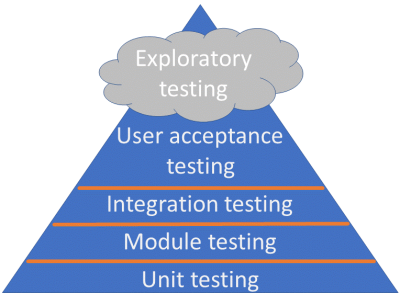
\includegraphics[scale=0.45]{triangle3.png}
     \end{center}
\end{column}
\end{columns}
\bigskip


As part of the tests, there are usually (1) a set of tests against \textbf{known bad states} that should never be entered, and (2) a set of tests checking the system is currently in a known good state, also called \textbf{invariant tests}.
\bigskip


HEVM can help with finding ways to trigger \emph{all} known bad states and validate that invariants \emph{always} hold.



\end{frame}


\begin{frame}{What is HEVM}

Can run EVM bytecode concretely like geth, or can run EVM bytecode symbolically:
\begin{itemize}
\item Takes as input known bad state/invariant test
\item Examines all execution paths
\item Finds the set of requirements to reach them
\item Runs external tool (SMT solver) to find input to reach them
\item Displays call \& state needed to trigger the bad state/invalidate the invariant
\end{itemize}
\end{frame}

\begin{frame}[fragile=singleslide]{Symbolic Execution: Basics}
Say your code looks like this:
\begin{Verbatim}[frame=single, framerule=0.2mm, framesep=2mm,fontsize=\small]
function (uint a) public pure {
	uint b
	unchecked { b = a + 1;}
	assert(b > a);
}
\end{Verbatim}


HEVM can find the case where $a=0xffffff\ldots$ to trigger the assert due to roll-around. HEVM gives you the \textbf{exact call to reproduce the bug}. This way of using HEVM can find a \emph{known-bad state}.

\end{frame}

\begin{frame}[fragile=singleslide]{Symbolic Execution vs Fuzzing}
Say your code looks like this:

\begin{Verbatim}[frame=single, framerule=0.2mm, framesep=2mm,fontsize=\small]
function (uint a, uint b) public pure {	
	// solution: a = 10000983843024
	//           b = 9877982748934
	
	if (a * 2 + b == 29879950434982 &&
	    b / 2 == 4938991374467) {
		assert(false); // bad things happen
	}
}
\end{Verbatim}

Fuzzing never finds this edge-case. Symbolic execution always finds it.
\bigskip 

\textbf{In general, fuzzing is faster, but is incomplete. Symbolic execution is slower but complete.}

\end{frame}

\begin{frame}[fragile=singleslide]{Symbolic Execution: Invariant Checking}
You can describe \textbf{invariants} of your contract and write them as functions Then assert these functions every time the invariant must hold.
\begin{Verbatim}[frame=single, framerule=0.2mm, framesep=2mm,fontsize=\small]
function my_invariant() private pure returns inv {
	inv = ...calculate invariant...
}
	
function (uint a) public pure {
	require(my_invariant());
	... your function code here ....
	assert(my_invariant());
}
\end{Verbatim}

Here, instead of a known-bad state, we validate that we are always in state that matches our expectations.
\end{frame}	


\begin{frame}[fragile=singleslide]{Symbolic Execution: Equivalence Checking}
You can ask HEVM to check whether two implementations are equivalent
\bigskip
\\

\begin{minipage}[b]{0.45\textwidth}
\begin{Verbatim}[frame=single, framerule=0.2mm, framesep=2mm,fontsize=\small]
function (...) public {
  simple known good
  function
  /uses lots of gas/
}
    \end{Verbatim}
  \end{minipage}
  \begin{minipage}[b]{0.45\textwidth}
  \begin{Verbatim}[frame=single, framerule=0.2mm, framesep=2mm,fontsize=\small]
function (...) public {
  complicated function
  
  /uses less gas/
}
\end{Verbatim}
\end{minipage}

HEVM can give you the exact \textbf{call to trigger the discrepancy} between the two functions. This way, you can safely improve the gas performance of your code.
\end{frame}




\begin{frame}[fragile=singleslide]{Limitations of HEVM}
While HEVM aims to be fully-featured, it has a number of inherent limitations:

\begin{itemize}
\item Loops can be challenging. The option \texttt{--max-iterations N} can raise the iteration limit until which loops are examined.
\item Recursion, and parametric calls can cause HEVM to only partially explore the state
\item Complicated mathematical expressions such as exponentiation can pose a challenge.
\item It is important to set all known invariants at the start of the test via \texttt{require()} to speed up solving.
\item HEVM itself is not verified, and neither are the solvers we use. However, some solvers will in the future be able to emit a proof, which can be verified.
\end{itemize}
\end{frame}

\begin{frame}[fragile=singleslide]{How it works: The Intermediate Representation}
\small

Through the interpreter we create the global expression that captures all end-states. We then take each end-state out and filter it for things we are looking for, e.g. assertion failures. This is our intermediate representation, similar to what YUL is for Solidity. Let's take the previous example:


\begin{Verbatim}[frame=single, framerule=0.2mm,framesep=2mm,fontsize=\small]
function (uint a) public pure {
	uint b
	unchecked { b = a + 1;}
	assert(b > a);
}
\end{Verbatim}

The expression to generate a counterexamle for this could look like:

\begin{Verbatim}[frame=single, framerule=0.2mm, framesep=2mm,fontsize=\small]
PLEq (Add (Var "a") (Lit 1)) (Var "a")
\end{Verbatim}

Notice: we use less-or-equal, because we want a \textbf{counterexample}
\end{frame}

\begin{frame}[fragile=singleslide]{How it Works: Passing the Expression to an SMT solver}

Let's say the expression is:

\begin{Verbatim}[frame=single, framerule=0.2mm, framesep=2mm,fontsize=\footnotesize]
PLEq (Add (Var "a") (Lit 1)) (Var "a")
\end{Verbatim}
\bigskip

The SMT expression for this could be:

\begin{Verbatim}[frame=single, framerule=0.2mm, framesep=2mm,fontsize=\footnotesize]
(set-logic QF_AUFBV)
(define-sort Word () (_ BitVec 256))
(declare-const varA (Word))
(assert (bvule (bvadd varA (_ bv1 256)) varA))
(check-sat)
\end{Verbatim}

Z3 gives the answer:

\begin{Verbatim}[frame=single, framerule=0.2mm, framesep=2mm,fontsize=\footnotesize]
sat
(
  (define-fun varA () (_ BitVec 256)
    #xffffffffffffffffffffffffffffffffffffffffffffffffffffffffffffffff)
)
\end{Verbatim}
\end{frame}

\section{How to Use and Contribute}
\begin{frame}[fragile=singleslide]{Using HEVM}

Install foundry [1]. Get static HEVM binary [2]. Install z3 [3]. Add foundry test cases, and prepend with \texttt{prove} the ones you want HEVM to run:

\begin{Verbatim}[frame=single, framerule=0.2mm, framesep=2mm,fontsize=\footnotesize]
function prove_add(uint x, uint y) public pure {
    unchecked { if (x + y < x) return; }
    assert(x + y >= x);
}
\end{Verbatim}

Then run with:

\begin{Verbatim}[frame=single, framerule=0.2mm, framesep=2mm,fontsize=\footnotesize]
forge build
hevm test
\end{Verbatim}


\bigskip

[1] \url{https://github.com/foundry-rs/foundry}

[2] \url{https://github.com/ethereum/hevm/releases}

[3] \url{https://github.com/Z3Prover/z3}
\end{frame}


\begin{frame}[fragile=singleslide]{Contributing Benchmarks}
To test and improve the performance of HEVM, we use a benchmark repository [1]. Here, you can test your example problem against other full-featured symbolic execution engines such as Halmos [2]:


\begin{Verbatim}[frame=single, framerule=0.2mm, framesep=2mm,fontsize=\footnotesize]
sh <(curl -L https://nixos.org/nix/install) --daemon
git clone https://github.com/eth-sc-comp/benchmarks/
nix develop
./bench.py
./gen_graphs.py
cd graphs
\end{Verbatim}

We are keen on in real-world benchmarks that you feel could be interesting for the community.

\bigskip

[1] \url{https://github.com/eth-sc-comp/benchmarks/}

[2] \url{https://github.com/a16z/halmos}
\end{frame}


\begin{frame}[fragile=singleslide]{Contributing Back to HEVM}

The HEVM repository uses\texttt{nix} for ease of development:

\begin{Verbatim}[frame=single, framerule=0.2mm, framesep=2mm,fontsize=\footnotesize]
sh <(curl -L https://nixos.org/nix/install) --daemon
git clone https://github.com/ethereum/hevm/
nix-shell
cabal run exe:hevm -- test
\end{Verbatim}

You now have a full development environment, with all necessary tools installed, including Z3.
\bigskip 

HEVM is written in Haskell, but there are many areas that can be contributed to without deep knowledge of Haskell. For example, expression simplification:

\begin{Verbatim}[frame=single, framerule=0.2mm, framesep=2mm,fontsize=\footnotesize]
    go (Add a b)
      | b == (Lit 0) = a
      | a == (Lit 0) = b
      | otherwise = add a b
\end{Verbatim}
\end{frame}

\section{Conclusions}
\begin{frame}{Conclusions}

HEVM is a fully-featured, easy-to-use tool that can help find bugs in your code. It can be a useful \textbf{part of your testing strategy}.
\bigskip

HEVM can help you gain more confidence in the correctness of your system. It can be especially helpful to validate that certain catastrophic failure modes cannot be triggered. HEVM, however, can be incomplete: it can struggle with loops, complicated/recursive call chains, and complicated mathematical expressions.
\bigskip

Download HEVM from \url{https://github.com/ethereum/hevm/releases}
\smallskip

\qrcode{https://github.com/ethereum/hevm/releases}

\end{frame}



\end{document}
